\documentclass[../main.tex]{subfiles}
\graphicspath{{\subfix{../Images/}}}
\begin{document}
\section{Graphing Techniques}

\subsection{Graph Features}
\subsubsection{Basic characteristics}
\textbf{Axial Intercepts}
\begin{align*}
    x-intercept \, &: \, y=0 \\
    y-intercept \, &: \, x=0 \\
\end{align*}
\textbf{Stationary Points} \\
Stationary points are points on a curve where \\
\[\frac{dy}{dx}\bigg|_{x=k}=0, \, k \in \mathbb{R}\]
The Nature of the stationary point can be determined by \\
using the second or first derivative tests \\\\
\textbf{Asymptotes} \\
A Line or curve that a function approaches arbitrarily \\
close to
\begin{align*}
    \text{Horizontal : when } &x \to \infty, \, y \to a, \text{where } a \in \mathbb{R} \; \therefore y=a \\
    \text{Vertical : when } &y \to \infty, \, x \to b, \text{where } b \in \mathbb{R} \; \therefore x=b  \\
    \text{Oblique : when } &x \to \infty, \, y \to cx+d, \text{where } c,d \in \mathbb{R} \\
                           &\therefore y=cx+d
\end{align*}
A Horizontal Asymptote can be cut through, but vertical \\
asymptotes will never be passed through

\subsubsection{Symmetry}
\textbf{Symmetric about the x-axis} \\
If \((x,y)\) is a point on the curve, \\
\((x,-y)\) will also be a point on the curve \\
\begin{tikzpicture}[scale=0.5]
    \draw[->] (-1,0) -- (10,0) node[right] {\(x\)};
    \draw[->] (0,-3.5) -- (0,3.5) node[above] {\(y\)};
    \draw[scale=1,domain=0:9,smooth,variable=\x,blue] plot ({\x},{sqrt(0.5*\x)});
    \draw[scale=1,domain=0:9,smooth,variable=\x,blue] plot ({\x},{-sqrt(0.5*\x)});
    \filldraw (4,1.414) circle (0.1) node[below right] {\((x,y)\)};
    \filldraw (4,-1.414) circle (0.1) node[above right] {\((x,-y)\)};
\end{tikzpicture} \newpage \noindent
\textbf{Symmetric about the y-axis (Even Functions)} \\
Mathematically, \(f(x)=f(-x)\) \\
\begin{tikzpicture}[scale=0.5]
    \draw[->] (-2*pi-0.5,0) -- (2*pi+0.5,0) node[right] {\(x\)};
    \draw[->] (0,-3.5) -- (0,3.5) node[above] {\(y\)};
    \draw[domain=-2*pi:2*pi,smooth,variable=\x,blue] plot ({\x},{3*cos(0.5*\x r)});
    \filldraw (-0.667*pi,1.5) circle (0.1) node[above left] {\((-x,y)\)};
    \filldraw (0.667*pi,1.5) circle (0.1) node[above right] {\((x,y)\)};
\end{tikzpicture} \\
\textbf{Symmetric about the origin (Odd Functions)} \\
Mathematically, \(f(x)=-f(x)\) \\
\begin{tikzpicture}[scale=0.5]
    \draw[->] (-2*pi-0.5,0) -- (2*pi+0.5,0) node[right] {\(x\)};
    \draw[->] (0,-3.5) -- (0,3.5) node[above] {\(y\)};
    \draw[domain=-2*pi:2*pi,smooth,variable=\x,blue] plot ({\x},{3*sin(0.25*\x r)});
    \filldraw (-0.667*pi,-1.5) circle (0.1) node[above left] {\((-x,-y)\)};
    \filldraw (0.667*pi,1.5) circle (0.1) node[below right] {\((x,y)\)};
\end{tikzpicture}


\subsection{Types of Graphs}
\subsubsection{Power Functions}
\boxed{\text{General Power Function : }f(x)=ax^{n}, \, a \in \mathbb{R}^{+}} \\\\
\textbf{When n is an even positive integer}
\begin{align*}
    \text{Function Type : } &\text{Even Function} \\
    \text{Common Points : } &(-1,a), \, (0,0), \, (1,a)
\end{align*}
\begin{tikzpicture}[scale=0.75]
    \draw[->] (-4.5,0) -- (4.5,0) node[right] {\(x\)};
    \draw[->] (0,-0.5) -- (0,5) node[above] {\(y\)};
    \draw[domain=-4:4,smooth,variable=\x,blue] plot ({\x},{(0.5*\x)^2});
    \filldraw (2,1) circle (0.1) node[above left] {\((-1,a)\)};
    \filldraw (-2,1) circle (0.1) node[above right] {\((1,a)\)};
\end{tikzpicture} \newpage \noindent
\textbf{When n is an odd positive integer, n \(\geq\) 3}
\begin{align*}
    \text{Function Type : } &\text{Odd Function} \\
    \text{Common Points : } &(-1,-a), \, (0,0), \, (1,a)
\end{align*}
\begin{tikzpicture}[scale=0.75]
    \draw[->] (-4.5,0) -- (4.5,0) node[right] {\(x\)};
    \draw[->] (0,-4.5) -- (0,4.5) node[above] {\(y\)};
    \draw[domain=-4:4,smooth,variable=\x,blue] plot ({\x},{(0.4*\x)^3});
    \filldraw (3,1.728) circle (0.1) node[above left] {\((1,a)\)};
    \filldraw (-3,-1.728) circle (0.1) node[below right] {\((-1,-a)\)};
\end{tikzpicture} \\\\
\textbf{When n is an even negative integer}
\begin{align*}
    \text{Function Type : } &\text{Even Function} \\
    \text{Common Points : } &(-1,a), \, (0,0), \, (1,a) \\
    \text{Horizontal Asymptote : } &y=0 \\
    \text{Vertical Vertical : } &x=0
\end{align*}
\begin{tikzpicture}[scale=0.75]
    \draw[->] (-4.5,0) -- (4.5,0) node[right] {\(x\)};
    \draw[->] (0,-0.5) -- (0,3) node[above] {\(y\)};
    \draw[domain=-4:-0.2,smooth,variable=\x,blue] plot ({\x},{-1/(\x*2)});
    \draw[domain=0.2:4,smooth,variable=\x,blue] plot ({\x},{1/(\x*2)});
    \filldraw (1,0.5) circle (0.1) node[above right] {\((1,a)\)};
    \filldraw (-1,0.5) circle (0.1) node[above left] {\((-1,a)\)};
\end{tikzpicture} \newpage \noindent
\textbf{When n is an odd negative integer}
\begin{align*}
    \text{Function Type : } &\text{Odd Function} \\
    \text{Common Points : } &(-1,-a), \, (0,0), \, (1,a) \\
    \text{Horizontal Asymptote : } &y=0 \\
    \text{Vertical Vertical : } &x=0
\end{align*}
\begin{tikzpicture}[scale=0.75]
    \draw[->] (-4.5,0) -- (4.5,0) node[right] {\(x\)};
    \draw[->] (0,-3) -- (0,3) node[above] {\(y\)};
    \draw[domain=-4:-0.2,smooth,variable=\x,blue] plot ({\x},{1/(\x*2)});
    \draw[domain=0.2:4,smooth,variable=\x,blue] plot ({\x},{1/(\x*2)});
    \filldraw (1,0.5) circle (0.1) node[above right] {\((1,a)\)};
    \filldraw (-1,-0.5) circle (0.1) node[below left] {\((-1,-a)\)};
\end{tikzpicture} \\\\\\
\textbf{When \(n \in \mathbb{Q}\) in the form \(\displaystyle \frac{1}{k}\) \\ Such that \(k\) is an even positive integer}
\begin{align*}
    \text{Common Points : } &(0,0), \, (1,a) \\
\end{align*}
\begin{tikzpicture}[scale=0.75]
    \draw[->] (-0.5,0) -- (8.5,0) node[right] {\(x\)};
    \draw[->] (0,-0.5) -- (0,3.5) node[above] {\(y\)};
    \draw[domain=0:8,smooth,samples=100,variable=\x,blue] plot ({\x},{\x^0.5});
\end{tikzpicture} \\
\textbf{When \(n \in \mathbb{Q}\) in the form \(\displaystyle \frac{1}{k}\) \\ Such that \(k\) is an odd positive integer}
\begin{align*}
    \text{Function Type : } &\text{Odd Function} \\
    \text{Common Points : } &(-1,-a), \, (0,0), \, (1,a) \\
\end{align*}
\begin{tikzpicture}[scale=0.75]
    \draw[->] (-4.5,0) -- (4.5,0) node[right] {\(x\)};
    \draw[->] (0,-2) -- (0,2) node[above] {\(y\)};
    \draw[domain=-4:4,smooth,samples=100,variable=\x,blue] plot ({\x},{\x^(1/3)});
    \filldraw (1,1) circle (0.1) node[below right] {\((1,a)\)};
    \filldraw (-1,-1) circle (0.1) node[above left] {\((-1,-a)\)};
\end{tikzpicture} \\
\subsubsection{Piecewise Functions}
Different intervals each has a different definition \\
\[
f(x) = \begin{cases}
    H(x), & \text{if } a \leq x < b \\
    G(x), & \text{if } b \leq x < c \\
    Q(x), & \text{Otherwise}
\end{cases}
\]
\begin{tikzpicture}[scale=0.75]
    \draw[->] (-4.5,0) -- (4.5,0) node[right] {\(x\)};
    \draw[->] (0,-4) -- (0,4) node[above] {\(y\)};
    \draw[domain=-4:-2,smooth,variable=\x,blue] plot ({\x},{0.25*\x});
    \draw[domain=-2:0,smooth,variable=\x,orange] plot ({\x},{0.5*\x^2});
    \draw[domain=0:2,smooth,samples=100,variable=\x,red] plot ({\x},{\x^(1/3)});
    \draw[domain=2:4,smooth,variable=\x,blue] plot ({\x},{0.25*\x});
    \filldraw (-2,-2) circle (0.1);
    \draw (-2,-0.5) circle (0.1);
    \draw (2,1.26) circle (0.1);
    \filldraw (2,0.5) circle (0.1);
\end{tikzpicture} \\
When the function is \textbf{discontinuous} between intervals, \\
A \textbf{Solid} dot is used if the point is on the \\
interval, an \textbf{empty} is used if it isn't \\\\
When the function is \textbf{Continuous} between intervals, \\
dots are not needed

\subsubsection{Periodic Functions}
A function that repeats itself after an interval, \\
Mathematically, \(f(x+\alpha)=f(x)\), where \(\alpha \in \mathbb{R}\) \\
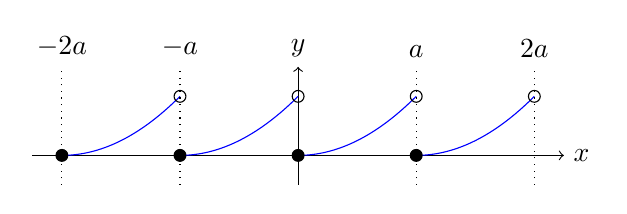
\begin{tikzpicture}[scale=0.75]
    \draw[->] (-4.5,0) -- (4.5,0) node[right] {\(x\)};
    \draw[->] (0,-0.5) -- (0,1.5) node[above] {\(y\)};
    \draw[domain=-4:-2,smooth,variable=\x,blue] plot ({\x},{(0.5*(4+\x))^2});
    \draw[domain=-2:0,smooth,variable=\x,blue] plot ({\x},{(0.5*(2+\x))^2});
    \draw[domain=0:2,smooth,variable=\x,blue] plot ({\x},{(0.5*\x)^2});
    \draw[domain=2:4,smooth,variable=\x,blue] plot ({\x},{(0.5*(\x-2))^2});

    % Dotted Lines between repetitions
    \draw[dotted] (-4,-0.5) -- (-4,1.5) node[above] {\(-2a\)};
    \draw[dotted] (-2,-0.5) -- (-2,1.5) node[above] {\(-a\)};
    \draw[dotted] (2,-0.5) -- (2,1.5) node[above] {\(a\)};
    \draw[dotted] (4,-0.5) -- (4,1.5) node[above] {\(2a\)};

    % Filled and Hollow circles to mark the included and unincluded points
    \filldraw (-4,0) circle (0.1);
    \filldraw (-2,0) circle (0.1);
    \filldraw (0,0) circle (0.1);
    \filldraw (2,0) circle (0.1);
    \draw (-2,1) circle (0.1);
    \draw (0,1) circle (0.1);
    \draw (2,1) circle (0.1);
    \draw (4,1) circle (0.1);
\end{tikzpicture} \\
In this example, the function \(f(x)\) had an interval of \\
\(0 \leq x < a\) \newpage \noindent

\subsubsection{Rational Functions}
A rational function is in the form \(\displaystyle y=\frac{p(x)}{q(x)}\), \\*
where \(p(x), q(x)\) are polynomials \\
\textbf{Types of Rational Functions} \\
\underline{Degree of \(p(x) \, <\) Degree of \(q(x)\)} \\
\(y=0\) is the Horizontal Asymptote \\
Solutions to \(q(x)=0\) will yield the Vertical Asymptote(s) \\\\
\underline{Degree of \(p(x)\) \(\geq\) Degree of \(q(x)\)} \\
\(\displaystyle y=\frac{p(x)}{q(x)} \equiv y=h(x)+\frac{r(x)}{q(x)}\), where \(deg(r(x)) < deg(q(x))\) \\
\(y=h(x)\) is the Oblique Asymptote \\
Solutions to \(q(x)=0\) will yield the Vertical Asymptote(s) \\\\
\textbf{Rectangular Hyperbola} \\
Rectangular Hyperbola : \(\displaystyle y=\frac{ax+b}{cx+d} \implies y=p+\frac{r}{cx+d}\), \\
where \(c \neq 0, x \neq -\frac{d}{c}\). The possible curve shapes are \\
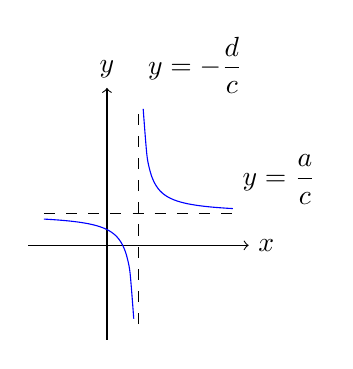
\begin{tikzpicture}[scale=0.4]
    \draw[->] (-2.5,0) -- (4.5,0) node[right] {\(x\)};
    \draw[->] (0,-3) -- (0,5) node[above] {\(y\)};
    %Graph%
    \draw[domain=-2:1-0.15,smooth,variable=\x,blue] plot ({\x},{1+1/(2*\x-2)});
    \draw[domain=1+0.15:4,smooth,variable=\x,blue] plot ({\x},{1+1/(2*\x-2)});

    % Asymptotes %
    \draw[dash pattern=on 4pt off 4pt] (-2,1) -- (4,1) node[above right] {\(\displaystyle y=\frac{a}{c}\)};
    \draw[dash pattern=on 4pt off 4pt] (1,-2.5) -- (1,4.5) node[above right] {\(\displaystyle y=-\frac{d}{c}\)};
\end{tikzpicture} \\
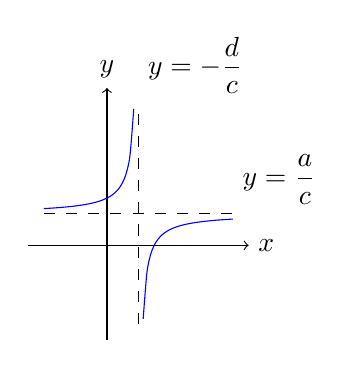
\begin{tikzpicture}[scale=0.4]
    \draw[->] (-2.5,0) -- (4.5,0) node[right] {\(x\)};
    \draw[->] (0,-3) -- (0,5) node[above] {\(y\)};
    %Graph%
    \draw[domain=-2:1-0.15,smooth,variable=\x,blue] plot ({\x},{1-1/(2*\x-2)});
    \draw[domain=1+0.15:4,smooth,variable=\x,blue] plot ({\x},{1-1/(2*\x-2)});

    % Asymptotes %
    \draw[dash pattern=on 4pt off 4pt] (-2,1) -- (4,1) node[above right] {\(\displaystyle y=\frac{a}{c}\)};
    \draw[dash pattern=on 4pt off 4pt] (1,-2.5) -- (1,4.5) node[above right] {\(\displaystyle y=-\frac{d}{c}\)};
\end{tikzpicture} \\
The Function is first to be rationalized by long division,
then the Asymptotes and graph features can be found with the information above \newpage \noindent
\textbf{Quadratic Over Linear Functions} \\
\(\displaystyle y=\frac{ax^2+bx+c}{dx+f} \implies y=px+q+\frac{r}{dx+f}\)
\begin{align*}
    \displaystyle \text{One Oblique Asymptote} \, &: \, y=px+q \\
    \displaystyle \text{One Vertical Asymptote} \, &: \, x=-\frac{f}{d}
\end{align*}
\underline{Case 1 : Two Turning Points} \\
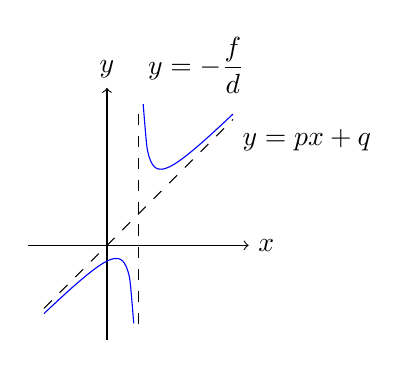
\begin{tikzpicture}[scale=0.4]
    \draw[->] (-2.5,0) -- (4.5,0) node[right] {\(x\)};
    \draw[->] (0,-3) -- (0,5) node[above] {\(y\)};
    %Graph%
    \draw[domain=-2:1-0.15,smooth,variable=\x,blue] plot ({\x},{\x+1/(2*\x-2)});
    \draw[domain=1+0.15:4,smooth,variable=\x,blue] plot ({\x},{\x+1/(2*\x-2)});

    % Asymptotes %
    \draw[dash pattern=on 4pt off 4pt] (-2,-2) -- (4,4) node[below right] {\(y=px+q\)};
    \draw[dash pattern=on 4pt off 4pt] (1,-2.5) -- (1,4.5) node[above right] {\(\displaystyle y=-\frac{f}{d}\)};
\end{tikzpicture} \\
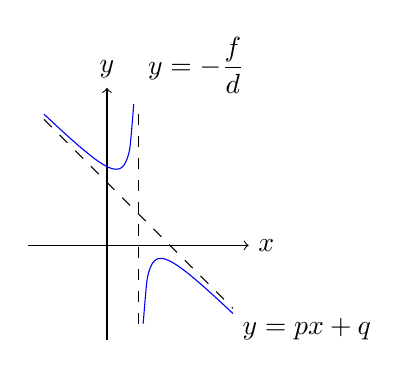
\begin{tikzpicture}[scale=0.4]
    \draw[->] (-2.5,0) -- (4.5,0) node[right] {\(x\)};
    \draw[->] (0,-3) -- (0,5) node[above] {\(y\)};
    %Graph%
    \draw[domain=1+0.15:4,smooth,variable=\x,blue] plot ({\x},{-\x+2+1/(-2*\x+2)});
    \draw[domain=-2:1-0.15,smooth,variable=\x,blue] plot ({\x},{-\x+2+1/(-2*\x+2)});

    % Asymptotes %
    \draw[dash pattern=on 4pt off 4pt] (-2,4) -- (4,-2) node[below right] {\(y=px+q\)};
    \draw[dash pattern=on 4pt off 4pt] (1,-2.5) -- (1,4.5) node[above right] {\(\displaystyle y=-\frac{f}{d}\)};
\end{tikzpicture} \\\\
\underline{Case 2 : No Turning Points} \\
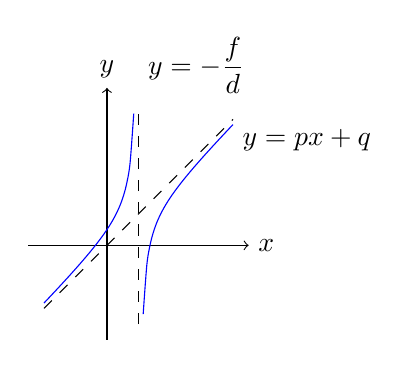
\begin{tikzpicture}[scale=0.4]
    \draw[->] (-2.5,0) -- (4.5,0) node[right] {\(x\)};
    \draw[->] (0,-3) -- (0,5) node[above] {\(y\)};
    %Graph%
    \draw[domain=-2:1-0.15,smooth,variable=\x,blue] plot ({\x},{\x-1/(2*\x-2)});
    \draw[domain=1+0.15:4,smooth,variable=\x,blue] plot ({\x},{\x-1/(2*\x-2)});

    % Asymptotes %
    \draw[dash pattern=on 4pt off 4pt] (-2,-2) -- (4,4) node[below right] {\(y=px+q\)};
    \draw[dash pattern=on 4pt off 4pt] (1,-2.5) -- (1,4.5) node[above right] {\(\displaystyle y=-\frac{f}{d}\)};
\end{tikzpicture} \\
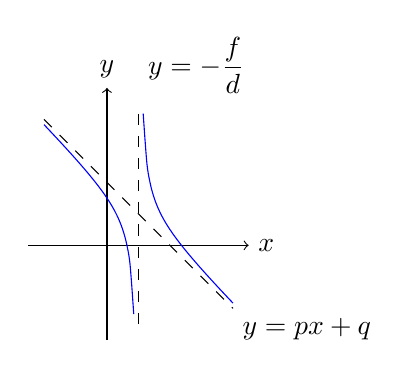
\begin{tikzpicture}[scale=0.4]
    \draw[->] (-2.5,0) -- (4.5,0) node[right] {\(x\)};
    \draw[->] (0,-3) -- (0,5) node[above] {\(y\)};
    %Graph%
    \draw[domain=1+0.15:4,smooth,variable=\x,blue] plot ({\x},{-\x+2-1/(-2*\x+2)});
    \draw[domain=-2:1-0.15,smooth,variable=\x,blue] plot ({\x},{-\x+2-1/(-2*\x+2)});

    % Asymptotes %
    \draw[dash pattern=on 4pt off 4pt] (-2,4) -- (4,-2) node[below right] {\(y=px+q\)};
    \draw[dash pattern=on 4pt off 4pt] (1,-2.5) -- (1,4.5) node[above right] {\(\displaystyle y=-\frac{f}{d}\)};
\end{tikzpicture} \newpage \noindent
\textbf{Linear Over Quadratic Functions} \\
\(\displaystyle y=\frac{dx+f}{ax^2+bx+c} \implies y=0+{dx+f}{ax^2+bx+c}\)
\begin{align*}
    \displaystyle \text{One Horizontal Asymptote} \, &: \, y=0 \\
    \displaystyle \text{Vertical Asymptote(s)} \, &: \, \text{Solve for denominator} = 0 \\
                                                  &| \,\,\,\, \text{Solutions} = \text{Asymptote(s)}
\end{align*}
\underline{Example : When there are 2 Vertical Asymptotes} \\
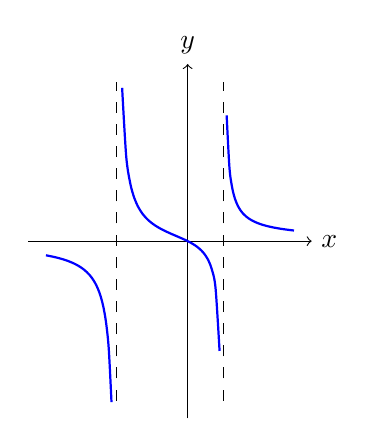
\begin{tikzpicture}[scale=0.45]
    \draw[->] (-4.5,0) -- (3.5,0) node[right] {\(x\)};
    \draw[->] (0,-5) -- (0,5) node[above] {\(y\)};

    % Plot the function
    \draw[blue, thick, domain=-4:-2-0.15, smooth, variable=\x] plot ({\x},{\x/((\x)^2+\x-2)});
    \draw[blue, thick, domain=-2+0.15:1-0.1, smooth, variable=\x] plot ({\x},{\x/((\x)^2+\x-2)});
    \draw[blue, thick, domain=1+0.1:3, smooth, variable=\x] plot ({\x},{\x/((\x)^2+\x-2)});

    % Asymptotes %
    \draw[dash pattern=on 4pt off 4pt] (1,-4.5) -- (1,4.5);
    \draw[dash pattern=on 4pt off 4pt] (-2,-4.5) -- (-2,4.5);
\end{tikzpicture}

\subsubsection{Reciprocal Functions}
\begin{tabularx}{0.5\textwidth} {
    | >{\centering\arraybackslash}X
    | >{\centering\arraybackslash}X | }
    \hline
    \textbf{\(y=f(x)\)} & \textbf{\(\displaystyle y=\frac{1}{f(x)}\)} \\
    \hline
    \(x\)-intercept : \(x=a\)  & Vertical Asymptote : \(x=a\)  \\
    \hline
    *Vertical Asymptote : \(x=a\)  & *\(x\)-intercept : \(x=a\)  \\
    \hline
    \((a,b)\)  & **\(\displaystyle \left(a,\frac{1}{b}\right)\)  \\
    \hline
    Local Maxima : \((a,b)\)  & Local Minima : **\(\displaystyle \left(a,\frac{1}{b}\right)\)  \\
    \hline
    Local Minima : \((a,b)\)  & Local Maxima : **\(\displaystyle \left(a,\frac{1}{b}\right)\)  \\
    \hline
    Horizontal Asymptote : \(y=b\)   & Horizontal Asymptote : \(\displaystyle y=\frac{1}{b}\)  \\
    \hline
    Oblique Asymptote : \(y=ax+b\)  & Horizontal Asymptote : \(y=0\)  \\
    \hline
    \(f(x)\) is increasing  & \(\displaystyle \frac{1}{f(x)}\) is decreasing  \\
    \hline
    \(f(x)\) is decreasing  & \(\displaystyle \frac{1}{f(x)}\) is increasing  \\
    \hline
  \end{tabularx} \\\\
* True for \textbf{most} cases \\
** \(b \neq 0\) \\\\
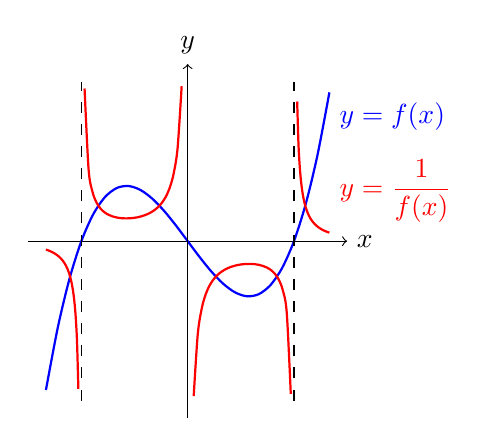
\begin{tikzpicture}[scale=0.45]
    \draw[->] (-4.5,0) -- (4.5,0) node[right] {\(x\)};
    \draw[->] (0,-5) -- (0,5) node[above] {\(y\)};

    % Plot the function
    \draw[blue, thick, domain=-4:4, smooth, variable=\x] plot ({\x},{0.15*(\x-3)*(\x)*(\x+3)}) node[below right] {\(y=f(x)\)};

    % Reciprocal function
    \draw[red, thick, domain=-4:-3-0.085, smooth, variable=\x] plot ({\x},{1/(0.15*(\x-3)*(\x)*(\x+3))});
    \draw[red, thick, domain=-3+0.09:-0.17, smooth, variable=\x] plot ({\x},{1/(0.15*(\x-3)*(\x)*(\x+3))});
    \draw[red, thick, domain=0.17:3-0.09, smooth, variable=\x] plot ({\x},{1/(0.15*(\x-3)*(\x)*(\x+3))});
    \draw[red, thick, domain=3+0.09:4, smooth, variable=\x] plot ({\x},{1/(0.15*(\x-3)*(\x)*(\x+3))}) node[above right] {\(\displaystyle y=\frac{1}{f(x)}\)};

    % Asymptotes %
    \draw[dash pattern=on 4pt off 4pt] (-3,-4.5) -- (-3,4.5);
    \draw[dash pattern=on 4pt off 4pt] (0,-4.5) -- (0,4.5);
    \draw[dash pattern=on 4pt off 4pt] (3,-4.5) -- (3,4.5);
\end{tikzpicture}


\subsection{Linear Transformations}
\subsubsection{Translation}
\underline{\(y=f(x-a)\)}
\begin{itemize}
    \item Translation of the graph \(f(x)\) by \(a\) units in the direction of the \(x\)-axis
    \item Add \(a\) to all of the \(x\)-coordinates
\end{itemize}
\underline{\(y=f(x-a)\)}
\begin{itemize}
    \item Translation of the graph \(f(x)\) by \(-a\) units in the direction of the \(x\)-axis
    \item Subtract \(a\) to all of the \(x\)-coordinates
\end{itemize}
\underline{\(y=f(x)+a\) or \(y-a=f(x)\)}
\begin{itemize}
    \item Translation of the graph \(f(x)\) by \(a\) units in the direction of the \(y\)-axis
    \item Add \(a\) to all of the \(y\)-coordinates
\end{itemize}
\underline{\(y=f(x)-a\) or \(y+a=f(x)\)}
\begin{itemize}
    \item Translation of the graph \(f(x)\) by \(-a\) units in the direction of the \(y\)-axis
    \item Subtract \(a\) to all of the \(y\)-coordinates
\end{itemize}
\newpage

\subsubsection{Scaling}
\underline{\(\displaystyle y=f\left(\frac{x}{a}\right)\)}
\begin{itemize}
    \item Scaling the graph \(f(x)\) by a scale factor of \(a\) parallel to the \(x\)-axis
    \item Multiply \(a\) to all of the \(x\)-coordinates
\end{itemize}
\underline{\(y=af(x)\) or \(\displaystyle \frac{y}{a}=f(x)\)}
\begin{itemize}
    \item Scaling the graph \(f(x)\) by a scale factor of \(a\) parallel to the \(y\)-axis
    \item Multiply \(a\) to all of the \(y\)-coordinates
\end{itemize}

\subsubsection{Reflection}
\underline{\(y=f(-x)\)}
\begin{itemize}
    \item Reflecting the graph \(f(x)\) about \(y\)-axis
    \item Multiply \(-1\) to all of the \(x\)-coordinates
\end{itemize}
\underline{\(y=-f(x)\)}
\begin{itemize}
    \item Reflecting the graph \(f(x)\) about \(x\)-axis
    \item Multiply \(-1\) to all of the \(y\)-coordinates
\end{itemize}

\subsubsection{Modulus Transformations}
\underline{\(y=|f(x)|\)}
\begin{itemize}
    \item Reflect the graph \(f(x)\) about \(y\)-axis \\* for the regions \textbf{below the \(x\)-axis}
    \item Multiply \(-1\) to the \(y\)-coordinates of the \\* \textbf{reflected points}
\end{itemize}
\underline{\(y=f(|x|)\)}
\begin{itemize}
    \item Remove the graph that is in the \textbf{negative \(x\)-axis} \\* Reflect the remaining graph \(f(x)\) about \(y\)-axis
    \item Multiply \(-1\) to the \(x\)-coordinates of the \\* \textbf{reflected points}
\end{itemize}
\underline{\(|y|=f(x)\)}
\begin{itemize}
    \item Remove the graph that is in the \textbf{negative \(y\)-axis} \\* Reflect the remaining graph \(f(x)\) about \(x\)-axis
    \item Multiply \(-1\) to the \(y\)-coordinates of the \\* \textbf{reflected points}
\end{itemize}
\newpage \noindent

\subsubsection{Sequence of Tranformations}
\underline{Suggested Sequence to minimise errors:}
\begin{enumerate}
    \item \(T_{x}\) \textbf{Horizontal} Translation
    \item \(S_{x}\) \textbf{Horizontal} Scaling
    \item \(S_{y}\) \textbf{Vertical} Scaling
    \item \(T_{y}\) \textbf{Vertical} Translation
\end{enumerate}
\boxedeq{\text{Sequence : } T_{x}S_{x}S_{y}T_{y}}

\subsection{Conic Sections}

\subsubsection{Ellipses}
\boxedeq{\text{Standard Form : } \frac{(x-h)^{2}}{a^{2}} + \frac{(y-k)^{2}}{b^{2}} = 1}
\begin{tikzpicture}[scale=0.75]
    \draw[->] (-0.5,0) -- (6,0) node[right] {\(x\)};
    \draw[->] (0,-0.5) -- (0,4) node[above] {\(y\)};
    %Graph
    \draw (3,2) ellipse (2 and 1);

    % Radius arrows
    \draw[<->] (1,2) -- (3,2) node[midway, above] {\(a\)};
    \draw[<->] (3,2) -- (3,1) node[midway, right] {\(b\)};

    % Center
    \filldraw (3,2) circle (2pt) node[above right] {\((h,k)\)};
\end{tikzpicture} \\
\underline{Properties}
\begin{itemize}
    \item Center : \((h,k)\)
    \item Semi-Major-Axis : \(a\)
    \item Semi-Minor-Axis : \(b\)
    \item Symmetrical about \(x=h\) \& \(y=k\)
\end{itemize}
\newpage \noindent

\subsubsection{Circles}
\boxedeq{\text{Standard Form : } (x-h)^{2} + (y-k)^{2} = 1}
\begin{tikzpicture}[scale=0.75]
    \draw[->] (-0.5,0) -- (6,0) node[right] {\(x\)};
    \draw[->] (0,-0.5) -- (0,4) node[above] {\(y\)};
    %Graph
    \draw (3,2) circle (1.5);

    % Radius arrows
    \draw[<->] (1.5,2) -- (3,2) node[midway, above] {\(a\)};
    \draw[<->] (3,2) -- (3,0.5) node[midway, right] {\(a\)};

    % Center
    \filldraw (3,2) circle (2pt) node[above right] {\((h,k)\)};
\end{tikzpicture} \\
\underline{Properties}
\begin{itemize}
    \item Center : \((h,k)\)
    \item Radius : \(a\)
    \item Symmetrical about \(x=h\) \& \(y=k\)
\end{itemize}

\subsubsection{Hyperbolas}
\boxedeq{\text{Standard Form : } \frac{(x-h)^{2}}{a^{2}} - \frac{(y-k)^{2}}{b^{2}} = 1}
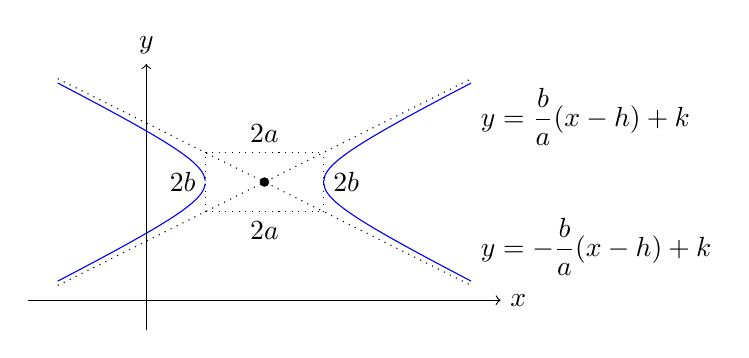
\begin{tikzpicture}[scale=0.75]
    \draw[->] (-2,0) -- (6,0) node[right] {\(x\)};
    \draw[->] (0,-0.5) -- (0,4) node[above] {\(y\)};
    %Graph
    \draw[blue] plot[domain=-1.5:1,samples=100] ({\x},{0.5*sqrt((\x-2)^2 - 1) + 2});
    \draw[blue] plot[domain=-1.5:1,samples=100] ({\x},{-0.5*sqrt((\x-2)^2 - 1) + 2});
    \draw[blue] plot[domain=3:5.5,samples=100] ({\x},{0.5*sqrt((\x-2)^2 - 1) + 2});
    \draw[blue] plot[domain=3:5.5,samples=100] ({\x},{-0.5*sqrt((\x-2)^2 - 1) + 2});

    % Dotted Box
    \draw[dotted] (1,2-0.5) -- (3,2-0.5) node[midway, below] {\(2a\)};
    \draw[dotted] (1,2+0.5) -- (3,2+0.5) node[midway, above] {\(2a\)};
    \draw[dotted] (1,2-0.5) -- (1,2+0.5) node[midway, left] {\(2b\)};
    \draw[dotted] (3,2-0.5) -- (3,2+0.5) node[midway, right] {\(2b\)};

    % Asymptotes
    \draw[dotted] (-1.5,0.25) -- (5.5,3.75) node[below right] {\(\displaystyle y=\frac{b}{a}(x-h)+k\)};
    \draw[dotted] (-1.5,3.75) -- (5.5,0.25) node[above right] {\(\displaystyle y=-\frac{b}{a}(x-h)+k\)};

    % Center
    \filldraw (2,2) circle (2pt);
\end{tikzpicture} \\
\underline{Properties}
\begin{itemize}
    \item Center : \((h,k)\)
    \item Symmetrical about \(x=h\) \& \(y=k\)
    \item Vertices are '\(b\)' units from the center \((h,k)\) \\* Vertically
    \item Oblique Asymptotes are \(\displaystyle y=\pm\frac{b}{a}(x-h)+k\)
\end{itemize}

\newpage \noindent

\boxedeq{\text{Standard Form : } \frac{(y-k)^{2}}{b^{2}} - \frac{(x-h)^{2}}{a^{2}} = 1}
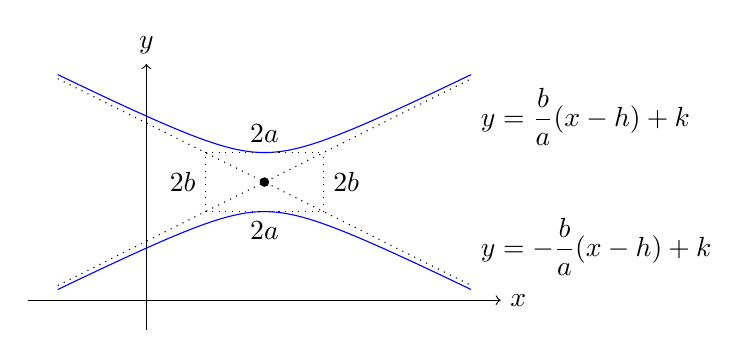
\begin{tikzpicture}[scale=0.75]
    \draw[->] (-2,0) -- (6,0) node[right] {\(x\)};
    \draw[->] (0,-0.5) -- (0,4) node[above] {\(y\)};
    %Graph
    \draw[blue] plot[domain=-1.5:5.5,samples=100] ({\x},{0.5*sqrt((\x-2)^2 + 1) + 2});
    \draw[blue] plot[domain=-1.5:5.5,samples=100] ({\x},{-0.5*sqrt((\x-2)^2 + 1) + 2});

    % Dotted Box
    \draw[dotted] (1,2-0.5) -- (3,2-0.5) node[midway, below] {\(2a\)};
    \draw[dotted] (1,2+0.5) -- (3,2+0.5) node[midway, above] {\(2a\)};
    \draw[dotted] (1,2-0.5) -- (1,2+0.5) node[midway, left] {\(2b\)};
    \draw[dotted] (3,2-0.5) -- (3,2+0.5) node[midway, right] {\(2b\)};

    % Asymptotes
    \draw[dotted] (-1.5,0.25) -- (5.5,3.75) node[below right] {\(\displaystyle y=\frac{b}{a}(x-h)+k\)};
    \draw[dotted] (-1.5,3.75) -- (5.5,0.25) node[above right] {\(\displaystyle y=-\frac{b}{a}(x-h)+k\)};

    % Center
    \filldraw (2,2) circle (2pt);
\end{tikzpicture} \\
\underline{Properties}
\begin{itemize}
    \item Vertexes : \((h,k\pm b)\)
    \item Symmetrical about \(x=h\) \& \(y=k\)
    \item Vertices are '\(a\)' units from the center \((h,k)\) \\* Horizontally
    \item Oblique Asymptotes are \(\displaystyle y=\pm\frac{b}{a}(x-h)+k\)
\end{itemize}

\subsubsection{Parabolas}
\boxedeq{\text{Standard Form : } (x-h)^{2} = 4p(y-k)}
\underline{If \(p>0\)} \\
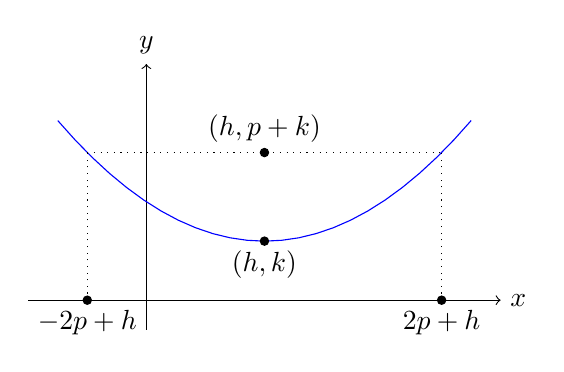
\begin{tikzpicture}[scale=0.75]
    \draw[->] (-2,0) -- (6,0) node[right] {\(x\)};
    \draw[->] (0,-0.5) -- (0,4) node[above] {\(y\)};
    %Graph
    \draw[blue] plot[domain=-1.5:5.5] ({\x},{((\x-2)^2)/6 + 1});

    % Vertex
    \filldraw (2,1) circle (2pt) node[below] {\((h,k)\)};

    % special points
    \filldraw (5,0) circle (2pt) node[below] {\(2p+h\)};
    \filldraw (-1,0) circle (2pt) node[below] {\(-2p+h\)};
    \filldraw (2,2.5) circle (2pt) node[above] {\((h,p+k)\)};

    % Dotted Lines
    \draw[dotted] (-1,0) -- (-1,2.5);
    \draw[dotted] (5,0) -- (5,2.5);
    \draw[dotted] (-1,2.5) -- (5,2.5);

\end{tikzpicture} \\\\
\underline{If \(p<0\)} \\
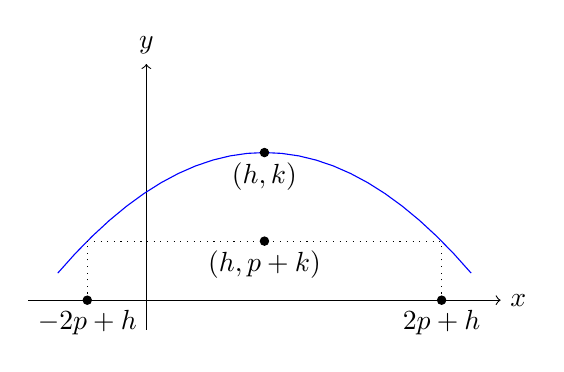
\begin{tikzpicture}[scale=0.75]
    \draw[->] (-2,0) -- (6,0) node[right] {\(x\)};
    \draw[->] (0,-0.5) -- (0,4) node[above] {\(y\)};
    %Graph
    \draw[blue] plot[domain=-1.5:5.5] ({\x},{-1*((\x-2)^2)/6 + 2.5});

    % Vertex
    \filldraw (2,2.5) circle (2pt) node[below] {\((h,k)\)};

    % special points
    \filldraw (5,0) circle (2pt) node[below] {\(2p+h\)};
    \filldraw (-1,0) circle (2pt) node[below] {\(-2p+h\)};
    \filldraw (2,1) circle (2pt) node[below] {\((h,p+k)\)};

    % Dotted Lines
    \draw[dotted] (-1,0) -- (-1,1);
    \draw[dotted] (5,0) -- (5,1);
    \draw[dotted] (-1,1) -- (5,1);

\end{tikzpicture}

\newpage \noindent
\underline{Properties}
\begin{itemize}
    \item Vertex : \((h,k)\)
    \item Symmetrical about \(x=h\)
    \item If \(p>0\), \(y\geq k\) \(\forall x (x \in \mathbb{R})\) \\* If \(p<0\), \(y\leq k\) \(\forall x (x \in \mathbb{R})\)
\end{itemize}

\boxedeq{\text{Standard Form : } (y-h)^{2} = 4p(x-k)}
\underline{If \(p>0\)} \\
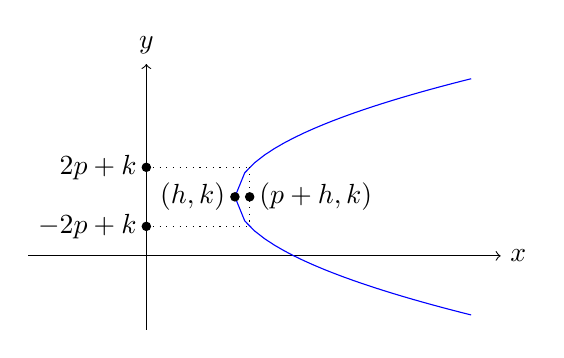
\begin{tikzpicture}[scale=0.75]
    \draw[->] (-2,0) -- (6,0) node[right] {\(x\)};
    \draw[->] (0,-1.25) -- (0,3.25) node[above] {\(y\)};
    %Graph
    \draw[blue] plot[domain=1.5:5.5] ({\x},{2*sqrt(0.25*(\x-1.5)) + 1});
    \draw[blue] plot[domain=1.5:5.5] ({\x},{-2*sqrt(0.25*(\x-1.5)) + 1});

    % Vertex
    \filldraw (1.5,1) circle (2pt) node[left] {\((h,k)\)};

    % special points
    \filldraw (0,1.5) circle (2pt) node[left] {\(2p+k\)};
    \filldraw (0,0.5) circle (2pt) node[left] {\(-2p+k\)};
    \filldraw (1.75,1) circle (2pt) node[right] {\((p+h,k)\)};

    % Dotted Lines
    \draw[dotted] (0,1.5) -- (1.75,1.5);
    \draw[dotted] (0,0.5) -- (1.75,0.5);
    \draw[dotted] (1.75,1.5) -- (1.75,0.5);

\end{tikzpicture} \\\\
\underline{If \(p<0\)} \\
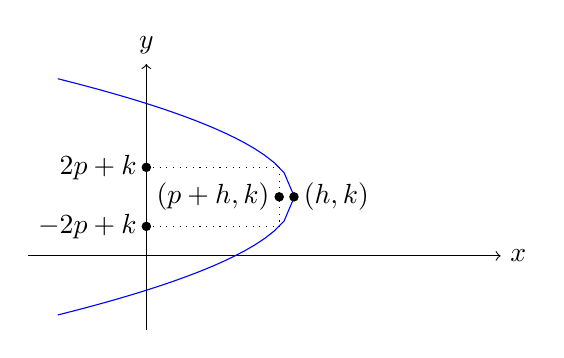
\begin{tikzpicture}[scale=0.75]
    \draw[->] (-2,0) -- (6,0) node[right] {\(x\)};
    \draw[->] (0,-1.25) -- (0,3.25) node[above] {\(y\)};
    %Graph
    \draw[blue] plot[domain=-1.5:2.5] ({\x},{2*sqrt(-0.25*(\x-2.5)) + 1});
    \draw[blue] plot[domain=-1.5:2.5] ({\x},{-2*sqrt(-0.25*(\x-2.5)) + 1});

    % Vertex
    \filldraw (2.5,1) circle (2pt) node[right] {\((h,k)\)};

    % special points
    \filldraw (0,1.5) circle (2pt) node[left] {\(2p+k\)};
    \filldraw (0,0.5) circle (2pt) node[left] {\(-2p+k\)};
    \filldraw (2.25,1) circle (2pt) node[left] {\((p+h,k)\)};

    % Dotted Lines
    \draw[dotted] (0,1.5) -- (2.25,1.5);
    \draw[dotted] (0,0.5) -- (2.25,0.5);
    \draw[dotted] (2.25,1.5) -- (2.25,0.5);

\end{tikzpicture} \\\\
\underline{Properties}
\begin{itemize}
    \item Vertex : \((h,k)\)
    \item Symmetrical about \(y=k\)
    \item If \(p>0\), \(x\geq h\) \(\forall y (y \in \mathbb{R})\) \\* If \(p<0\), \(x\leq h\) \(\forall y (y \in \mathbb{R})\)
\end{itemize}
\newpage \noindent

\subsection{Parametric Equations}
Expressing the variables of a function using another variable.
\begin{align*}
    \text{Cartesian Equation : }& f(x,y) \\
    \text{Parametric Equation : }& x=f(t) \text{ \& } y=f(t)
\end{align*}
\subsubsection{Sketching Parametric Curves (Using GC)}
Set an appropriate range for \(t\) under \textbf{Parametric} Mode \\
and key in the \(x(t)\) \& \(y(t)\) functions to graph it out \\
but draw a table of \(t\) and the respective \(x,y\) \\
\textbf{Table example:} \\
\begin{tabular}{ | c | c | c | c | }
    \hline
    \(t\) & -1 & 0 & 1 \\
    \hline
    \(x\) & 3 & 1 & 3 \\
    \hline
    \(y\) & -4 & 1 & 2 \\
    \hline
\end{tabular}

\subsubsection{Finding Asymptotes of Parametric Curves}
\underline{Example : \(\displaystyle x=\frac{1}{t}, \, y=t+1\) for \(t>0\)} \\\\
As \(y \to \infty\), \(t \to \infty\) \(\implies x \to 0\) \\* \(\therefore x=0\) is a Horizontal Asymptote \\
As \(x \to \infty\), \(t \to 0\) \(\implies y \to 1\) \\* \(\therefore y=1\) is a Vertical Asymptote \\\\
\(t\) acts as an intermediary

\subsubsection{Conversion of Parametric to Cartesian Equations}
Manipulate the terms containing the additional variable \\*
(such as \(t\)) until it can be cancelled out to give an equation \\*
with only the original variables. Trig Identities can be used too. \\\\
\underline{Example : \(x=a\cos{t}\), \(y=a\sin{t}\)}
\begin{align*}
    \displaystyle x^{2} &= a^{2}\left(1-\sin^{2}{t}\right) \\
    \displaystyle x^{2} &= a^{2} - a^{2}\left(\frac{y^{2}}{a^{2}}\right) \\
    \displaystyle \therefore y^{2} + x^{2} &= a^{2} \text{  [Cartesian Equation]}
\end{align*}

\end{document}